\graphicspath{{Chapter0-Introduction/}}
\chapter{Introduction}
\label{chap0:intro}

Galaxies are the most immediately visible large structures in the universe, broadly containing some combination of stars, stellar remnants, gas, and dark matter. Though the relative abundances of baryons and dark matter are thought to have been set almost immediately after the Big Bang, the proportions of gas, stars, and stellar remnants in a single galaxy are deeply informative about the individual. In other words, galaxies' properties can be inferred largely from the light emitted by stars and gas. With this information, observers may discern a galaxy's history and fate.

The process of galaxy evolution can be envisaged as the transformation of cold gas into stars, and the subsequent recycling of the stars' ejecta (rich in elements heaver than Helium---``metals") back into the a galaxy's ambient gaseous reservoir. This process begins after the initial collapse of a dark matter halo, with the progenitors of more massive dark matter halos (corresponding to denser regions in the early universe) collapsing, accreting baryons, and forming stars first. Each subsequent generation of stars builds upon the metal ejecta of generations before. Consequently, the dark matter halos most depleted in their supply of cold, neutral gas have a larger proportion of heavy elements. Metal content is described in two major ways: the first, common in stellar astrophysics, quantifies a mass fraction of all metals (and is notated $Z$). The chemistry of the interstallar medium (ISM) is described by the abundance of oxygen, by number, in relation to hydrogen on a logarithmic scale (notated \OonH). The chemistry of the interstellar medium is sensitive to the total star-formation that has occured throughout a galaxy's lifetime, and is of the most pertinence to this dissertation.

\section{Problems in galaxy chemical evolution}

Early theories of galaxy formation relied upon the idea that a single cloud of primordial gas formed a single galaxy \citep{eggen_62}. Therefore, the gas fraction ($f_g = \frac{M_{\textrm{gas}}}{M_{\textrm{gas}} + M_*}$) should be a simple and reliable indicator of evolutionary state, giving information about the galaxy's past star-formation and its potential to form stars in the future \citep{tinsley_80_chemev,pei_fall_95}. In this theory, a galaxy was a ``closed box" which neither gained nor lost gas, but simply transformed its original gas reservoir into stars until the gas ran out.

Today we know that the actual picture is more complicated: galaxies form hierarchically and from the ``inside-out" \citep{wang_kauffmann_11,bovy_16}---meaning that galaxy centers collapsed and formed stars earlier in cosmic time, and disks formed as gas built up around the bulge. Feedback from supernovae gives rise to gas and metal transport within galaxies, as well as more wholesale expulsion of gas from the disk \citep[``galactic winds"][]{veilleux_15_winds}. In simulations, bursty star-formation drives brief, ``gusty" outflows that eject much of the interstellar medium from the galaxy disk, briefly suppressing further star formation and enriching the circum-galactic medium \citep[CGM,][]{muratov_15_gusty}. This idea is also borne out by case-studies of, e.g., NGC891, which exhibits an \textsc{Hi} disk in profile preferentially ``puffed-up" in regions with the most vigorous star formation \citep{oosterloo_07_ngc891}. However, it is not clear whether this gas eventually rains back down onto the disk (a ``galactic fountain"), or simply remains in the halo. Figure \ref{fig:GasFlows} shows the gas flows thought to impact galaxies' ongoing chemical evolution.

\begin{figure}[H]
    \centering
    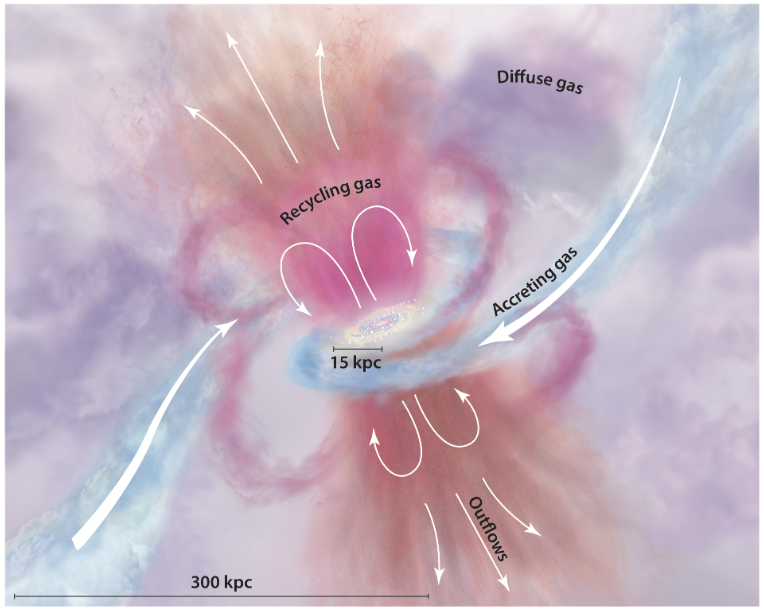
\includegraphics[width=\textwidth]{gasflows_tumlinson}
    \caption[A cartoon of the multiphase gas flows around galaxies]{\fixspacing A cartoon representation of the multiphase gas flows present near a star-forming galaxy, reproduced from \citet{tumlinson_peeples_werk_CGMreview}. Gas, some combination of metal-enriched and pristine, forms stars; and the mechanical \& radiation feedback from the most massive stars drives outflows into the halo while further metal-enriching the ambient gas.}
	\label{fig:GasFlows}
\end{figure}

It is likely that gas not only flows out of galaxies, but also in. The simplest reason is to allow star-formation to proceed for many Gyr. For the Milky Way's current star-formation rate (SFR) to continue unabated for the past 8 Gyr without also exhausting the Galaxy's gaseous reservoir, additional gas must have been introduced at a similar rate ($1.5 ~ {\rm M_{\odot} yr^{-1}}$). This is also true of statistical samples of galaxies all the way back to the peak of the cosmic star-formation rate density \citep{tacconi_2013}. Even continued star-formation alone seems to demand consistent refueling. Exacerbating matters further is star-formation's self-regulating effects: the winds from massive stars and the mechanical impacts from the ensuing supernovae drive cold gas out of the disk at rates greater than the SFR \citep{chisholm_18_outflows, roberts-borsani_20_outflows}. The impact of star-formation on surrounding cold gas is much greater than simple depletion, and bolster the indirect arguments for continual infusions of new gas.

There are also chemical signatures of gaseous refueling: the distributions of metal abundances in Milky Way G-dwarf stars were long known to be inconsistent with the closed-box model of chemical evolution \citep{vandenbergh_62_gdwarf}, though the accepted resolution was much later to come: the ``G-dwarf problem" can be solved by allowing galaxies to accrete gas from other sources \citep{fraternali_07}. Indeed, observations of the Milky Way and other galaxies indicate that dwarf companions do contribute gas to their larger, nearby siblings \citep{martinez-delgado_2010}. The chemical abundances of this gas seems to be seeded by the original parent halo: \citet{schaefer_19_accretion} demonstrated the likely pre-enrichment of gas in low-mass satellites in higher-mass halos: in other words, low-mass galaxies have their metallicities ``seeded'' by gas accreted from the more massive galaxies in whose halos they reside. A simple ``re-budgeting'' of gas between galaxies does not accomplish the wholesale rejuvenation that will continually sustain star formation.

The supply of gas that galaxies can exchange with their neighbors is just a drop in the bucket compared to the gas residing outside galaxies. Simulations suggest that galaxies will accrete pristine gas in ``cold flows" along filaments between galaxies, the ``cosmic web" \citep{silk_mamon_2012,sancisi08,cresci_2010_accretion}. Recent observations of distant systems near the peak of the cosmic star formation rate density show gas kinematics suggestive of accretion from the cosmic web's gas reservoirs. Figure \ref{fig:kcwi_inflows} shows a simulated multi-filament inflow beside two Lyman-alpha emitter systems observed with the Keck Cosmic Web Imager integral-field unit \citep{martin_19_kcwi-inflows}. Those systems, at $z \sim 2.5$, are very different from the galaxies present in the local universe; but conceptually demonstrate that the gas in extragalactic filaments could be captured by galaxies and transformed into stars.

\begin{figure}
    \centering
    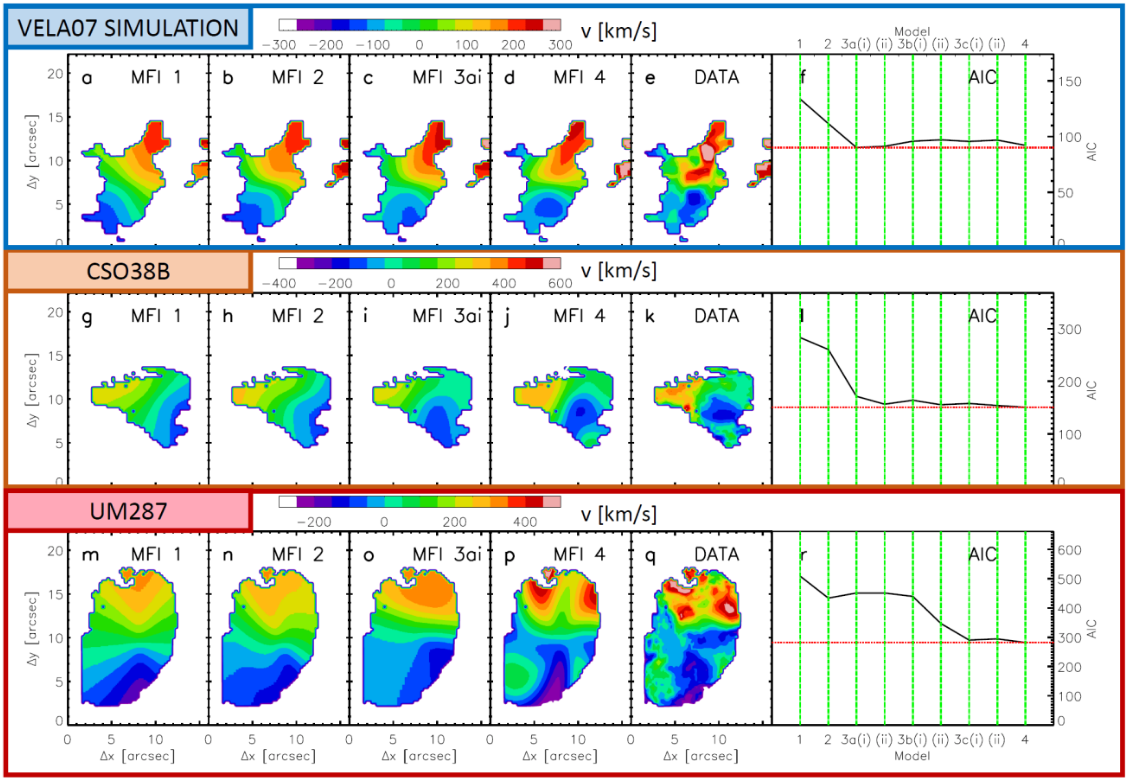
\includegraphics[width=\textwidth]{kcwi_inflows}
    \caption[Simulations and reported observations ($z \sim 2.5$) of multi-filament inflows]{\fixspacing Velocity maps of a simulated multi-component inflow impacting a star-forming disk (top row); and of two observed Lyman-alpha emitters (bottom two rows). Each system is fit by four models (left-most four columns in each row): Model 1 is a simple Keplerian disk in an NFW dark matter profile; Model 2 adds an isotropic radial collapse; Model 3ai replaces the radial collapse with a single collimated inflow; and Model 4 replaces the single inflow with a three-mode inflow, also adding azimuthal flows away from each source filament. The measured velocity map is shown in the second-from-right panel. The right-most panel shows the Akaike Information Criterion (AIC) for each model: this model diagnostic penalizes complex models. Despite these penalties, accretion from multiple sources is favored.}
    \label{fig:kcwi_inflows}
\end{figure}

\subsection{Chemical evolution: the theoretical \& the practical}

Though the co-evolution of gas fraction, metallicity, and stellar mass reflects a complex interplay between accretion, star formation, supernova- \& AGN-driven outflows, and galaxy-galaxy interactions, several robust, empirical relationships emerge: galaxies with higher gas fractions tend to have lower masses \citep{de-blok_96}, form rotationally-supported disks \citep{mcgaugh_de-blok_97}, and lie on the ``star-forming main sequence" (SFMS), a linear correlation between stellar mass and star-formation rate (SFR) \citep{brinchmann_04_sfms}. Additionally, a positive correlation is observed between galaxy mass and metal content (the mass-metallicity relation, or MZR) \citep{tremonti_mz}. When combined, these trends imply that galaxies' SFRs ``self-regulate", and so the process of galaxy-wide chemical enrichment is gradual \citep{finlator_dave_oppenheimer_12,fu_kauffmann_13}. Thus, even though the closed-box model of chemical evolution is not true in detail, gas fraction remains an illustrative property.

Galaxies' self-regulatory mechanisms bring about a sort of equilibrium. Yes, galaxies do evolve---but they do so slowly in comparison to the lifetimes of individual star-forming regions. Figure \ref{fig:gasreg_model} shows a cartoon of a chemical evolution model which treats instantaneous star-formation and evolving metallicity as quantities governed by a gas reservoir (this model and others like it have been termed ``gas-regulator models''---\citealt{lilly_13_gasreg, finlator_dave_oppenheimer_12}). In such models, the availability (or not) of gas drives star formation forward. The gaseous reservoir is depleted by the material residing in long-lived stars, as well as by the gaseous outflows which the massive, short-lived stars expel (``feedback''). Those same feedback mechanisms return metals to the reservoir, relocate them to other reservoirs, or banish them to the halo. Finally, the reservoir is rejuvenated by gas either originating from other reservoirs (in which case it has been processed through the star-formation and is metal-enriched) or from low-metallicity sources such as the cosmic web.

\begin{figure*}
    \centering
    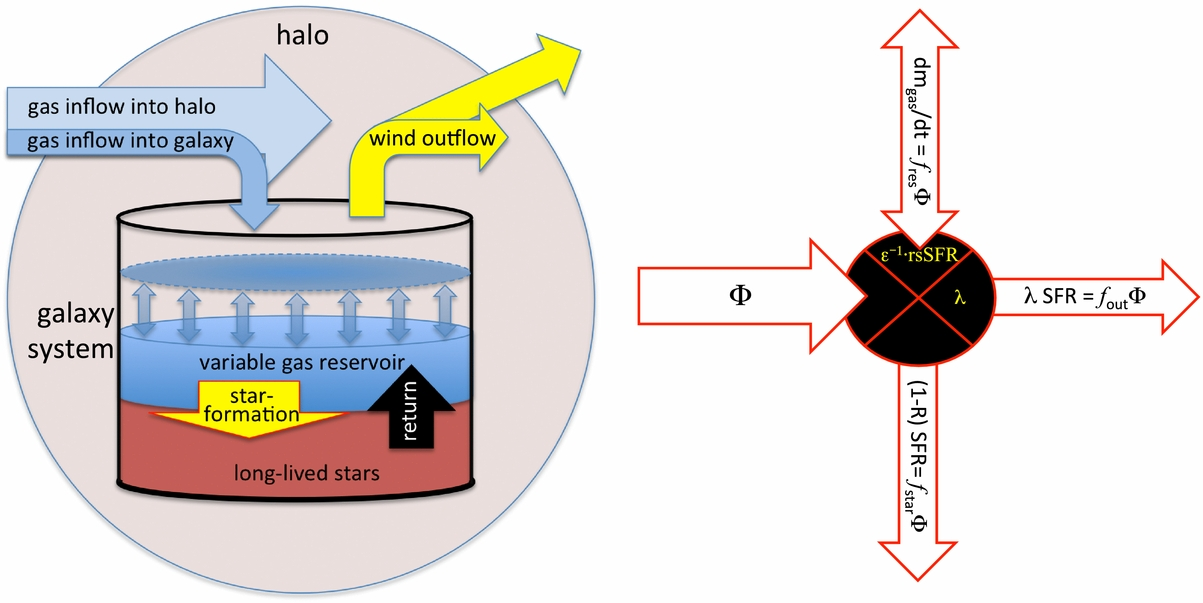
\includegraphics[width=\textwidth]{gasreg_model}
    \caption[A graphical representation of a gas-regulator or ``bathtub" model of chemical evolution]{\fixspacing A graphical representation of a gas-regulator or ``bathtub" model of chemical evolution, reproduced from \citet{lilly_13_gasreg}. Gas is introduced at a rate $\Phi$, and its exhaustion by star-formation \& winds, as well as its proportional return to the halo and disk, are dictated by the balance between $\Phi$, $\lambda, \epsilon$, and $R$, the parameters governing the gaseous inflow rate, the power of winds, the star-formation efficiency, and the mass fraction of old stars which do not produce appreciable quantities of metals.}
    \label{fig:gasreg_model}
\end{figure*}

\subsection{Inflows: where are they, and what are their effects?}

Measurements of the gas and metals \textit{lost} by star-forming galaxies due to feedback have become more possible with time \citep{telford_19_m31-metal-loss, chisholm_18_outflows, belfiore_vincenzo_maiolino_19}. The exact parameters of inflows in samples of galaxies remain elusive, though. The Milky Way's high-velocity clouds (HVCs) have long been considered signatures of the Galaxy's gas exchange with its environment: HVCs are gas clouds characterized by extreme velocities relative to the Milky Way disk, as well as relatively low metallicities (generally less than $0.5 ~ Z_{\odot}$), both of which suggest that they originated elsewhere and are now being accreted. HVCs may have analogs in the extragalactic context, but radio instrumentation has not reached the combination of resolution and sensitivity required to map them in relation to galaxies' ambient gas supply. Furthermore, though simulations indicate that the filaments of the cosmic web supply rejuvenating gas flows, the structures are orders of magnitude larger in size than galaxies and the medium much more diffuse and thus observationally inaccessible. It is worth repeating, though, that inflows are at least a buttress of current galaxy chemical evolution theories, if not a keystone. They must be understood and characterized, not merely inferred.

In order to deeply understand galaxies' self-regulation, we must measure their star-forming gaseous reservoirs. This is most straightforwardly accomplished using radio (21cm HI) observations. Indeed, radio follow-up of optical surveys is commonplace; however, it is very infrequently complete in either scope, resolution, or depth. All three are required to spot and statistically characterize inflows. Simply put, interferometric surveys have yet to be realized due to their inherent immense time commitment. For example, the highest-resolution configuration on the Very Large Array (A-array, which has beam size 2'') requires 5.5 hours on source to reach an RMS noise of 0.2 mJy ($N = 2.08 \times 10^{21} ~ {\rm cm^{-2}}$, or $\Sigma \sim  16 ~ {\rm M_{\odot} pc^{-2}}$) with a velocity resolution of 40 km s$^{-1}$. This is many times larger than the on-source time of the latest resolved spectroscopic surveys. There have been attempts to circumvent radio observations by using the optical attenuation (modulated by metallicity and an assumed dust-to-metal ratio) as a proxy for gas content \citep{brinchmann_13,carton_brinchmann_2017, barrera-ballesteros_20_edge-califa}, but the uncertainties, systematics, and degeneracies involved have not been fully quantified. In particular, low-metallicity inflows likely have very different dust content \citep{kahre_walterbos_2018_legus_dusttogas}. For the purposes of locating gaseous inflows, it is therefore most prudent to fall back on global estimates of gas content, such as single-dish HI surveys, whose samples are larger and more statistically complete.

\subsection{How to measure a galaxy's stellar mass}

A galaxy's mass in stars serves as a proxy for its evolutionary stage: as a general rule, the higher a galaxy's stellar mass, the earlier the progenitor dark matter halo collapsed, and the more evolved the system is at the present day. Measuring stellar mass is fraught with uncertainties, though, which emerge largely due to the variable brightnesses \& colors of different-age \& -mass stars. If every star's mass-to-light ratio was the same, then a precise measurement of total flux would yield a precise measurement of mass. Complicating the matter is the relative rarity of high-mass stars: if high-mass stars were the most abundant by number, a stellar population's luminosity would better reflect is mass. Thus, it can be observationally difficult to reliably disentagle the true balance between a galaxy's old and young stellar populations, when the most visible constituents are the youngest and brightest. 

Other factors also influence the light that reaches us from stellar populations. Figure \ref{fig:conroy_sps_figure} (reproduced from \citet{conroy_sps_review}) illustrates the inputs to stellar population synthesis (SPS), starting at models of individual stars \& their birth abundance by number, including their modulation by foreground dust, and culminating in a model of the spectral energy distribution (SED) of a composite stellar population (CSP, the weighted sum of many fixed-metallicity, coeval stellar populations). This process has many observational degeneracies, most importantly between stellar age, stellar metallicity, and foreground dust attenuation. Increasing any one of the three reddens a spectrum, but it is difficult to distinguish which of the three is responsible, and therefore, what the exact past SFH is.

\begin{figure}
    \centering
    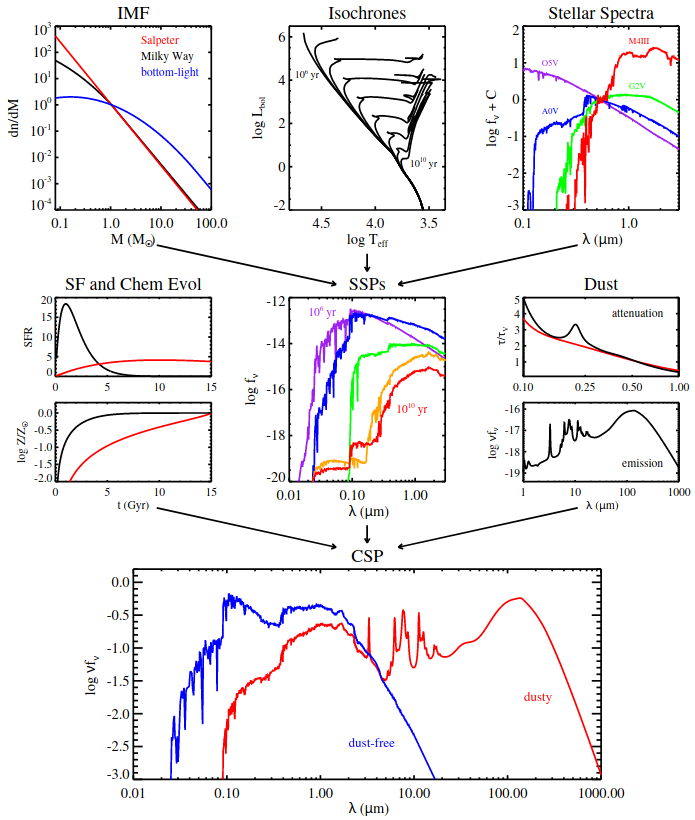
\includegraphics[width=\textwidth]{conroy_sps_review}
    \caption[A graphical overview of the components of stellar population synthesis.]{A graphical overview of the components of stellar population synthesis, reproduced from \citet{conroy_sps_review}. Three example stellar initial mass functions (IMFs) are shown in the upper left panel, several stellar isochrones ($10^6 - 10^10 ~ {\rm yr}$) are shown in the top center panel, and four individual stellar spectra are shown in the top right panel. These three components are combined to form simple stellar populations (SSPs, center panel), which are themselves modulated by a star-formation history (SFH, middle left panel). After attenuation by dust and addition of line emission (center right panel), a continuous stellar population (CSP) and its spectrum are yielded (bottom panel).}
    \label{fig:conroy_sps_figure}
\end{figure}

Some early attempts to disentangle stellar populations of different ages in the extragalactic context revolved around relations between optical colors and stellar mass-to-light ratios \citep[see][]{bell_dejong_01, bell_03}. These relations (CMLRs) were calibrated by assuming a star-formation history (generally exponentially-declining, a ``$\tau$ model''), a stellar IMF, and a set of isochrones and model stellar atmospheres. These relations yield adequate order-of-magnitude estimates for photometric observations, but their precision belies the systematics \& observational degeneracies at play. CSPs with very different star-formation histories can have very similar photometric signatures, since they may have a diversity of metallicities, balance of stellar ages, and foreground dust attenuation. With high-precision spectroscopic surveys, many (though not all) of these difficulties can be overcome. By precisely measuring a galaxy's stellar mass, one measures part of the denominator of gas fraction (or equivalently, further constrains the balance between young \& old stars), and quantifies a galaxy's evolutionary state.

\subsection{The growth of resolved spectroscopic surveys}



\section{Contents of this dissertation}

The aim of this dissertation is to track the buildup of stellar mass and metals in the gas phase across a large sample of galaxies with resolved spectroscopic measurements, and relate those to the availability \& ongoing consumption of star-forming gas. Chapter 2 endeavors to measure the stellar content of galaxies at kiloparsec scales. 
This is accomplished by quantifying the degeneracies in spectroscopic observations using a low-dimensional spectroscopic basis set generated with principal component analysis (PCA). The result is a catalog of resolved stellar mass maps for approximately 4700 galaxies. Chapter 3 compares the resolved mass estimates from Chapter 2 to measurements of galaxy dynamical masses obtained by studying the vertical kinematics of face-on disk galaxies; and aggregates \& aperture-corrects the maps of resolved stellar mass into a catalog of total galaxy stellar masses, also addressing the effects of resolution mismatch on estimates of stellar mass. This dissertation's final chapter, Chapter 4, turns to galaxies' gas-phase chemical abundances, and relates resolved chemistry to a galaxy's total gas content. We identify a correlation between a strongly-varying radial oxygen abundance profile, increased metallicity scatter at fixed radius, and enhanced HI content; and attempt to explain the extreme metallicities and gas content with atomic-rich, low-metallicity inflows from galaxies' environments. The intuitive model produces qualitative agreement with analytic models of chemical evolution in the presence of inflows; and may permit selection of probable inflow hosts for hig-resolution radio follow-up. Together, these three works expand the existing breadth of measurements of galaxy chemical evolution, and provide a path towards statistical characterization of galaxies' transformation through time.

\bibliographystyle{thesis.bst}
\bibliography{references}{}


%\clearpage
%\phantomsection % Fixes references link in hyperref/PDF index